\documentclass{standalone}

% graphics
\usepackage{tikz}
\usepackage{pgfplots}
\usepackage{siunitx}

\begin{document}

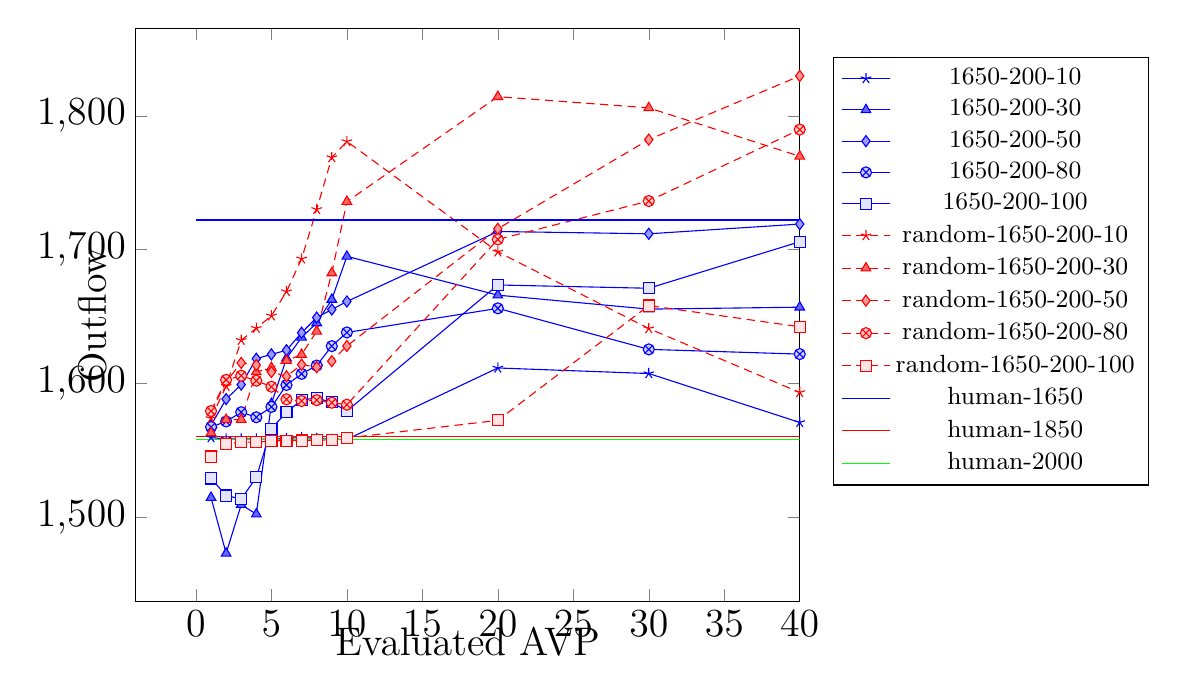
\begin{tikzpicture}[scale=1]
  \pgfplotsset{
      scale only axis,
      every x tick label/.append style={font=\Large},
      every y tick label/.append style={font=\Large},
	legend style={at={(1.05,0.95)},anchor=north west}
  }

\pgfplotscreateplotcyclelist{mycolorlist}{%
	blue,every mark/.append style={fill=blue!80}, mark=star, error bars/.cd, y dir=both, y explicit\\%
	blue,every mark/.append style={fill=blue!60}, mark=triangle*, error bars/.cd, y dir=both, y explicit\\%
	blue,every mark/.append style={fill=blue!40}, mark=diamond*, error bars/.cd, y dir=both, y explicit\\%
	blue,every mark/.append style={fill=blue!20}, mark=otimes*, error bars/.cd, y dir=both, y explicit\\%
	blue,every mark/.append style={fill=blue!10}, mark=square*, error bars/.cd, y dir=both, y explicit\\%
	red,densely dashed,every mark/.append style={solid,fill=red!80}, mark=star, error bars/.cd, y dir=both, y explicit\\%
	red,densely dashed,every mark/.append style={solid,fill=red!60},mark=triangle*, error bars/.cd, y dir=both, y explicit\\%
	red,densely dashed,every mark/.append style={solid,fill=red!40},mark=diamond*, error bars/.cd, y dir=both, y explicit\\%
	red,densely dashed,every mark/.append style={solid,fill=red!20}, mark=otimes*, error bars/.cd, y dir=both, y explicit\\%
	red,densely dashed,every mark/.append style={solid,fill=red!10}, mark=square*, error bars/.cd, y dir=both, y explicit\\%
	green!40!black, dashed,every mark/.append style={solid,fill=green!80}, mark=star, error bars/.cd, y dir=both, y explicit\\%
	green!40!black, dashed,every mark/.append style={solid,fill=green!60},mark=triangle*, error bars/.cd, y dir=both, y explicit\\%
	green!40!black, dashed,every mark/.append style={solid,fill=green!40},mark=diamond*, error bars/.cd, y dir=both, y explicit\\%
	green!40!black, dashed,every mark/.append style={solid,fill=green!20},mark=otimes*, error bars/.cd, y dir=both, y explicit\\%
	green!40!black, dashed,every mark/.append style={solid,fill=green!10},mark=square*, error bars/.cd, y dir=both, y explicit\\%
	black, dashed,every mark/.append style={solid,fill=green!80}, mark=star, error bars/.cd, y dir=both, y explicit\\%
	black, dashed,every mark/.append style={solid,fill=green!60},mark=triangle*, error bars/.cd, y dir=both, y explicit\\%
	black, dashed,every mark/.append style={solid,fill=green!40},mark=diamond*, error bars/.cd, y dir=both, y explicit\\%
	black, dashed,every mark/.append style={solid,fill=green!20},mark=otimes*, error bars/.cd, y dir=both, y explicit\\%
	black, dashed,every mark/.append style={solid,fill=green!10},mark=square*, error bars/.cd, y dir=both, y explicit\\%
	}


\begin{axis}[
    legend style={font=\small},
	ylabel={\Large Outflow},
	x label style={at={(axis description cs:0.5,-0.03)},anchor=north},
	y label style={at={(axis description cs:-0.030,0.5)}, anchor=south},
	xlabel={\Large Evaluated AVP},
	xmax=40,
	cycle list name=mycolorlist
]

\addplot table [x=a, y=b] {
a	 b	 c
1	1559.63	14.0
2	1558.76	13.35
3	1558.66	13.94
4	1558.62	14.12
5	1558.48	14.11
6	1559.05	13.68
7	1559.81	14.0
8	1559.05	14.41
9	1558.4	13.86
10	1558.33	13.45
20	1611.68	21.36
30	1607.54	19.0
40	1571.0	16.75
50	1543.57	19.19
60	1529.78	21.35
70	1515.35	18.77
80	1501.45	21.59
100	1483.74	24.48
};
\label{1650-200-10}

\addplot table [x=a, y=b] {
a	 b	 c
1	1514.88	16.63
2	1473.23	15.9
3	1509.59	25.95
4	1502.5	36.88
5	1584.97	32.75
6	1618.92	29.83
7	1634.51	25.39
8	1645.31	26.78
9	1662.84	32.19
10	1695.06	31.67
20	1666.08	40.67
30	1655.64	52.06
40	1657.08	60.04
50	1664.39	66.09
60	1669.32	67.79
70	1686.71	75.81
80	1685.81	66.97
100	1643.36	78.43
};
\label{1650-200-30}

\addplot table [x=a, y=b] {
a	 b	 c
1	1568.84	17.0
2	1588.43	16.72
3	1599.23	16.41
4	1618.6	19.01
5	1621.84	20.64
6	1624.9	22.16
7	1638.04	24.5
8	1649.34	24.59
9	1655.35	31.76
10	1661.33	37.64
20	1713.64	37.8
30	1711.91	48.81
40	1719.18	59.52
50	1722.17	63.88
60	1709.75	69.66
70	1704.35	57.54
80	1714.07	53.34
100	1709.32	61.11
};
\label{1650-200-50}

\addplot table [x=a, y=b] {
a	 b	 c
1	1567.58	15.35
2	1571.72	18.77
3	1578.64	20.01
4	1574.86	17.19
5	1582.6	21.71
6	1598.98	21.2
7	1607.29	20.35
8	1613.48	20.67
9	1627.99	23.51
10	1638.22	24.9
20	1656.22	19.89
30	1625.58	26.89
40	1622.05	41.43
50	1647.97	49.03
60	1676.12	60.18
70	1699.13	54.57
80	1702.98	48.1
100	1688.58	39.5
};
\label{1650-200-80}

\addplot table [x=a, y=b] {
a	 b	 c
1	1529.17	17.25
2	1516.39	25.91
3	1513.8	18.9
4	1529.96	30.13
5	1566.4	24.91
6	1578.56	23.38
7	1587.82	21.91
8	1589.22	22.43
9	1585.98	25.34
10	1579.54	24.53
20	1673.68	26.52
30	1671.23	40.74
40	1705.97	47.61
50	1727.93	54.24
60	1737.76	43.62
70	1733.26	43.23
80	1721.2	39.23
100	1683.68	38.33
};
\label{1650-200-100}

\addplot table [x=a, y=b] {
a	 b	 c
1	1574.03	17.33
2	1598.04	19.58
3	1632.38	22.39
4	1641.38	20.9
5	1650.67	24.6
6	1668.74	25.46
7	1693.22	27.09
8	1730.16	33.72
9	1768.86	34.18
10	1780.88	35.2
20	1698.41	39.87
30	1641.13	46.69
40	1593.4	55.7
50	1538.86	61.6
60	1474.16	69.98
70	1412.03	84.56
80	1347.3	90.21
100	1244.52	97.85
};
\label{random-1650-200-10}

\addplot table [x=a, y=b] {
a	 b	 c
1	1563.16	15.05
2	1573.09	16.57
3	1573.09	17.28
4	1608.73	19.73
5	1611.86	21.24
6	1617.16	19.83
7	1621.69	22.19
8	1639.08	29.47
9	1682.64	38.17
10	1735.96	37.0
20	1814.33	41.29
30	1805.98	33.97
40	1769.8	30.57
50	1733.62	34.44
60	1691.53	35.17
70	1633.21	38.76
80	1599.23	45.89
100	1505.34	57.09
};
\label{random-1650-200-30}

\addplot table [x=a, y=b] {
a	 b	 c
1	1578.64	15.1
2	1601.39	15.48
3	1615.43	18.22
4	1613.84	16.22
5	1608.66	17.38
6	1605.46	18.22
7	1614.17	18.84
8	1612.26	23.21
9	1616.72	27.41
10	1628.1	28.24
20	1715.65	39.88
30	1782.25	44.09
40	1829.81	40.72
50	1816.27	33.17
60	1800.18	28.49
70	1783.44	27.85
80	1759.39	24.09
100	1712.74	27.0
};
\label{random-1650-200-50}

\addplot table [x=a, y=b] {
a	 b	 c
1	1579.5	17.38
2	1602.79	14.3
3	1605.92	14.63
4	1602.18	17.06
5	1597.68	17.36
6	1588.28	15.8
7	1586.99	18.48
8	1587.64	20.31
9	1585.73	17.92
10	1584.25	22.83
20	1707.73	26.92
30	1736.39	46.23
40	1789.78	49.27
50	1816.88	46.87
60	1833.19	41.14
70	1837.98	31.18
80	1837.37	29.54
100	1810.26	25.74
};
\label{random-1650-200-80}

\addplot table [x=a, y=b] {
a	 b	 c
1	1545.52	20.24
2	1554.84	15.96
3	1556.35	15.48
4	1556.17	13.97
5	1557.22	14.98
6	1557.36	15.49
7	1557.47	13.69
8	1557.76	14.12
9	1557.9	14.66
10	1559.38	14.95
20	1572.55	21.39
30	1658.3	21.78
40	1642.46	28.68
50	1662.88	40.11
60	1737.32	48.93
70	1817.64	48.09
80	1819.15	28.01
100	1752.37	21.87
};
\label{random-1650-200-100}

\addplot[blue, samples=200] coordinates {(0,1722.200000) (100,1722.200000)};\label{human-1650}\addplot[red, samples=200] coordinates {(0,1560.380000) (100,1560.380000)};\label{human-1850}\addplot[green, samples=200] coordinates {(0,1558.120000) (100,1558.120000)};\label{human-2000}\addlegendimage{/pgfplots/refstyle=1650-200-10}
\addlegendentry{1650-200-10}
\addlegendimage{/pgfplots/refstyle=1650-200-30}
\addlegendentry{1650-200-30}
\addlegendimage{/pgfplots/refstyle=1650-200-50}
\addlegendentry{1650-200-50}
\addlegendimage{/pgfplots/refstyle=1650-200-80}
\addlegendentry{1650-200-80}
\addlegendimage{/pgfplots/refstyle=1650-200-100}
\addlegendentry{1650-200-100}
\addlegendimage{/pgfplots/refstyle=random-1650-200-10}
\addlegendentry{random-1650-200-10}
\addlegendimage{/pgfplots/refstyle=random-1650-200-30}
\addlegendentry{random-1650-200-30}
\addlegendimage{/pgfplots/refstyle=random-1650-200-50}
\addlegendentry{random-1650-200-50}
\addlegendimage{/pgfplots/refstyle=random-1650-200-80}
\addlegendentry{random-1650-200-80}
\addlegendimage{/pgfplots/refstyle=random-1650-200-100}
\addlegendentry{random-1650-200-100}
\addlegendimage{/pgfplots/refstyle=human-1650}
\addlegendentry{human-1650}
\addlegendimage{/pgfplots/refstyle=human-1850}
\addlegendentry{human-1850}
\addlegendimage{/pgfplots/refstyle=human-2000}
\addlegendentry{human-2000}


\end{axis}
\end{tikzpicture}
\end{document}
